%%%%%%%%%%%%%%%%%%%%%%%%%%%%%%%%%%%%%%%%%%%%%%%%%%%%%%%%%%%%%%%%%%%%%
%% This is a "template" model document for submission to the
%% American Chemical Society (ACS).
%%
%% The guidance here contains information about how you may wish to
%% modify it to match the requirements of various ACS journals. The
%% ACS do *not* typeset accepted articles using LaTeX, so there is
%% no specific class required.
%%
%% This template deliberately does *not* seek to reproduce
%% the layout of the typeset journal: this is explicitly not
%% required by the ACS for LaTeX submissions.
%%
%% Please report any issues with the template at
%% https://github.com/josephwright/acs-template/issues
%%
%% Released under the Creative Commons 0 license
%% https://creativecommons.org/public-domain/cc0/
%% 
%% Copyight (c) 2025 Joseph Wright
%%%%%%%%%%%%%%%%%%%%%%%%%%%%%%%%%%%%%%%%%%%%%%%%%%%%%%%%%%%%%%%%%%%%%
\documentclass[letterpaper]{article}

%%%%%%%%%%%%%%%%%%%%%%%%%%%%%%%%%%%%%%%%%%%%%%%%%%%%%%%%%%%%%%%%%%%%%
%% Font setup - delete if you are using LuaLaTeX
%%%%%%%%%%%%%%%%%%%%%%%%%%%%%%%%%%%%%%%%%%%%%%%%%%%%%%%%%%%%%%%%%%%%%
\usepackage[T1]{fontenc}

%%%%%%%%%%%%%%%%%%%%%%%%%%%%%%%%%%%%%%%%%%%%%%%%%%%%%%%%%%%%%%%%%%%%%
%% Adjust the margins and allow for line spacing
%%%%%%%%%%%%%%%%%%%%%%%%%%%%%%%%%%%%%%%%%%%%%%%%%%%%%%%%%%%%%%%%%%%%%
\usepackage{geometry}
\geometry{margin = 1in}
\usepackage{setspace}

%%%%%%%%%%%%%%%%%%%%%%%%%%%%%%%%%%%%%%%%%%%%%%%%%%%%%%%%%%%%%%%%%%%%%
%% Reference support
%%
%% The recommended method for producing the reference section is
%% to use biblatex. If you wish to use a classical BibTeX
%% approach, this is easiest to achieve using the achemso package.
%% In that case, you should remove the biblatex lines.
%%%%%%%%%%%%%%%%%%%%%%%%%%%%%%%%%%%%%%%%%%%%%%%%%%%%%%%%%%%%%%%%%%%%%
% You can adjust the printing of DOI, article title, etc. using
% package options, e.g. "doi = true"; see the biblatex manual for
% details of adjusting the number of authors printed, e.g.
% "maxnames = 15" to print no more than 15 authors.
% \usepackage[style = chem-acs]{biblatex}
% \addbibresource{pqe.bib}
% If you are using classical BibTeX, remove the above lines and 
% uncomment:
\usepackage{achemso}

%%%%%%%%%%%%%%%%%%%%%%%%%%%%%%%%%%%%%%%%%%%%%%%%%%%%%%%%%%%%%%%%%%%%%
%% Graphic inclusion and scheme and chart support3....
%%%%%%%%%%%%%%%%%%%%%%%%%%%%%%%%%%%%%%%%%%%%%%%%%%%%%%%%%%%%%%%%%%%%%
\usepackage{graphicx}
\usepackage{float}
\newfloat{scheme}{htbp}{los}
\floatname{scheme}{Scheme}
\floatname{chart}{Chart}
\newfloat{graph}{htbp}{loh}

%%%%%%%%%%%%%%%%%%%%%%%%%%%%%%%%%%%%%%%%%%%%%%%%%%%%%%%%%%%%%%%%%%%%%
%% Common support packages
%%%%%%%%%%%%%%%%%%%%%%%%%%%%%%%%%%%%%%%%%%%%%%%%%%%%%%%%%%%%%%%%%%%%%
\usepackage{chemformula} % Formulas using \ch{}
% or
\usepackage[version = 4]{mhchem} % Formulas using \ce{}

%%%%%%%%%%%%%%%%%%%%%%%%%%%%%%%%%%%%%%%%%%%%%%%%%%%%%%%%%%%%%%%%%%%%%
%% Many journals require that sections are unnumbered: this 
%% is activated here
%%%%%%%%%%%%%%%%%%%%%%%%%%%%%%%%%%%%%%%%%%%%%%%%%%%%%%%%%%%%%%%%%%%%%
\setcounter{secnumdepth}{-1}

%%%%%%%%%%%%%%%%%%%%%%%%%%%%%%%%%%%%%%%%%%%%%%%%%%%%%%%%%%%%%%%%%%%%%
%% Place any additional macros here.  Please use \newcommand* where
%% possible, and avoid layout-changing macros (which are not used
%% when typesetting).
%%%%%%%%%%%%%%%%%%%%%%%%%%%%%%%%%%%%%%%%%%%%%%%%%%%%%%%%%%%%%%%%%%%%%
\newcommand*\mycommand[1]{\texttt{\emph{#1}}}

%%%%%%%%%%%%%%%%%%%%%%%%%%%%%%%%%%%%%%%%%%%%%%%%%%%%%%%%%%%%%%%%%%%%%
%% Author and title data:
%% the authblk package is currently the simplest way to provide this
%%%%%%%%%%%%%%%%%%%%%%%%%%%%%%%%%%%%%%%%%%%%%%%%%%%%%%%%%%%%%%%%%%%%%
\usepackage{authblk}
\author[1]{Patryk Kozlowski}
\affil[1]{Department of Chemistry and Chemical Biology, Harvard University, Cambridge, MA 02138, USA}


\title{Theoretical Spectroscopy via Many-Body Perturbation Theory}

\begin{document}

\maketitle


%%%%%%%%%%%%%%%%%%%%%%%%%%%%%%%%%%%%%%%%%%%%%%%%%%%%%%%%%%%%%%%%%%%%%
%% Start the main part of the manuscript here.
%%%%%%%%%%%%%%%%%%%%%%%%%%%%%%%%%%%%%%%%%%%%%%%%%%%%%%%%%%%%%%%%%%%%%
\abstract{

The accurate prediction of spectroscopic properties is essential for materials discovery, motivating the development of efficient theoretical methods for excited states. Many-body perturbation theory (MBPT), formulated in terms of Green’s functions, offers a computationally attractive alternative to high-level wavefunction approaches such as equation-of-motion coupled-cluster theory. In this work, we examine MBPT-based methods for computing quasiparticle energies and spectral functions. First, we show that the moment-conserving GW (MCGW) method, despite its formal connection to Lanczos diagonalization, suffers from incurable numerical instabilities. We then study the spectral function of the uniform electron gas using the cumulant expansion, using second-order perturbation theory to improve upon the standard GW-based scheme. Lastly, we outline future directions, including self-consistent cumulant schemes and memory-kernel-based formulations.
}
\section{Introduction}
The consensus is that the best way to adapt to climate change is to mitigate it by reducing greenhouse gas emissions \cite{OECD2022-vn}. To do so requires the development of next-generation green technologies, such as electrocatalysts\cite{Seh2017-jx}, photovoltaics\cite{Du2023-kd}, and batteries\cite{Titirici2024-ao}. All of these seemingly disparate goals can be achieved through the discovery of materials with special properties. Spectroscopy is an indispensable tool for experimentalists in the search for such properties, as it illuminates the electronic structure of candidate materials. Computation is crucial for interpreting spectroscopic data and, therefore, quantum chemists devote a great deal of effort to the accurate and efficient simulation of spectra\cite{Neese2025-lp}. Spectroscopy occurs when incoming light perturbs matter, a process which proceeds through excited states of the system. The equation-of-motion coupled-cluster formalism including single and double excitations (EOM-CCSD) is able to provide an accurate description of excited states\cite{Krylov2008-sg}, but it carries a computational scaling of $O(N^6)$, where $N$ is the system size. A compelling alternative is presented by many-body perturbation theory (MBPT). MBPT introduces a variety of "gap-filling" methods, in the sense that these methods provide a description of excited states that is competitive with EOM-CCSD\cite{Golze2019-wm}, albeit with a lower computational cost. 


\section{Excited states via MBPT}
% Conceptually, MBPT describes quasiparticles. The quasiparticle of interest to me is the plasmon, which occurs due to collective excitations of electrons. This is because electonically excited states may be thought of in terms of the 
The native language of MBPT is that of Green's functions, which are used to describe the propagation of quasiparticles. The exact propagator is given by the interacting Green's function, $G$. The reference propagator is given by the noninteracting Green's function, $G_0$. The exact self-energy $\Sigma$ captures the difference between the two. However, solving for the exact quantities is computationally intractable, so approximations are necessary.

\subsection{Quasiparticle Energies from GW}
GW is a widely used approximation to the self-energy, which gets its name from postulating that $\Sigma$ is the product of the Green's function $G$ and the screened Coulomb interaction $W$ in the time domain, i.e. $\Sigma^{GW}(t) = i G(t) W(t)$. The GW method has been shown to give quasiparticle energies rivaling EOM-CCSD \cite{Bruneval2021-uj}. The most expensive part of a GW calculation is the computation of $\Sigma^{GW}$, as it requires an integration along the real frequency axis, which is ridden with poles. Avoiding these poles requires repeated use of Cauchy's residue theorem, incurring a computational scaling of $O(N^6)$. Therefore, analytic continuation (AC) is used, which computes $\Sigma^{GW}$ along that imaginary frequency axis and then analytically continues it to the real axis. This has the effect of reducing the scaling of a GW calculation to $O(N^4)$. However, the AC procedure becomes numerically unstable when computing quasiparticle energies of core states, which may be important for describing the system accurately\cite{Golze2019-wm}. Via a Löwdin partitioning technique, \citet{Quintero-Monsebaiz2022-en} showed that one can attain the exact quasiparticle energies within the GW approximation by either solving a nonlinear quasiparticle equation, as is traditionally done, or by determining the eigenvalues of an effective Hamiltonian, which we denote $\mathbf{H}^{\mathrm{GW}}$. However, an explicit construction of $\mathbf{H}^{\mathrm{GW}}$ carries the same $O(N^6)$ cost as solving the exact GW quasiparticle equation.

\citet{Scott2023-gc} claimed to have come up with a scheme for diagonalizing $\mathbf{H}^{\mathrm{GW}}$ at a low cost, by reformulating $\mathbf{H}^{\mathrm{GW}}$ in terms of the spectral moments of the self-energy. Considering self-energy moments to infinite order would be equivalent to constructing the full $\mathbf{H}^{\mathrm{GW}}$, but it is argued that truncating the moment expansion to some finite order yields a good approximation for a portion of the spectrum. A procedure inspired by the Lanczos algorithm is devised to iteratively diagonalize $\mathbf{H}^{\mathrm{GW}}$, with the Ritz values expected to rapidly converge to the ED solution as the number of moments increases. If one uses the resolution-of-the-identity (RI) approximation to the electron repulsion integrals, no step in this procedure scales higher than $O(N^4)$.

However, in my implementation, I found that the Ritz values do not always converge to the quasiparticle energies obtained by an exact diagonalization of $\mathbf{H}^{\mathrm{GW}}$ (ED@GW). The Lanczos algorithm is a well-established numerical method\cite{Lanczos1950-ox}, whose Ritz values are proven to converge to the eigenvalues of a matrix under proper conditions. One of these conditions requires that orthogonality be maintained in the Krylov subspace, which is typically done via periodic reorthogonalization. Figure~\ref{fig:mcgw_failure} shows how MCGW initially follows the Lanczos' convergence towards ED@GW, but then diverges. Analysis revealed that MCGW cannot perform reorthogonalization since it does not have access to its own Krylov subspace, leading to numerical instability. Therefore, we concluded that MCGW is an unusable method. A reliable quantum chemistry method should remain faithful to its theoretical foundation without ambiguity from numerical artifacts, ensuring that errors remain below other dominant sources such as basis set incompleteness and grid effects \cite{Pulay1980-bo}.

\begin{figure}[h!]
  \centering
  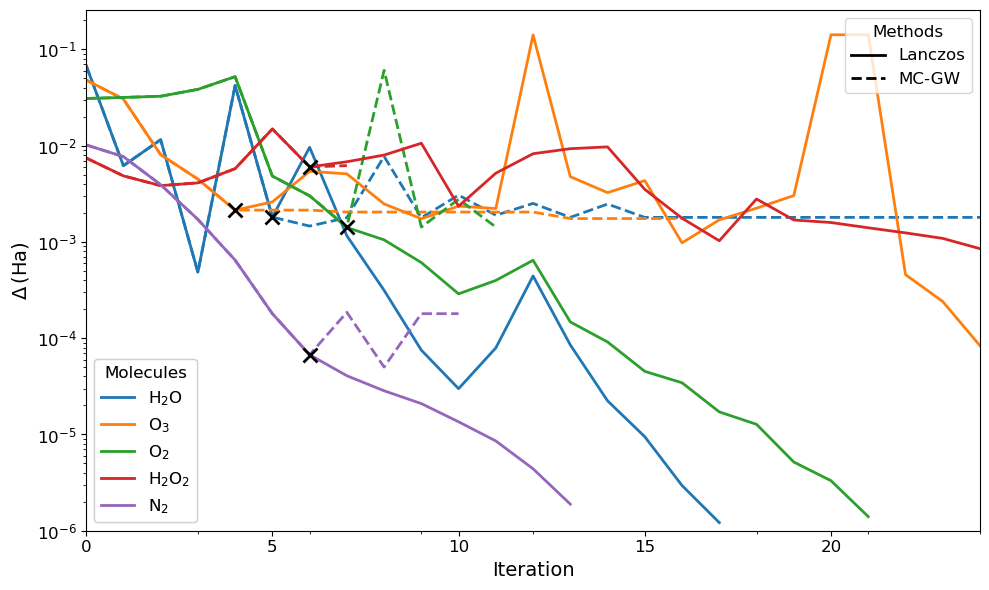
\includegraphics[width=0.75\textwidth]{../figs/mcgw_convergence_multi.png}
  \caption{Convergence of MCGW towards the GW quasiparticle energies of a variety of small molecules in the cc-pVDZ basis. $\Delta$ is the maximum difference between the ED@GW solution and the Ritz value of a given iteration in the pseudo-active space. This pseudo-active space is defined by the combination of all $N_{occ}$ orbitals plus the first $N_{occ}$ virtual orbitals. The desired numerical accuracy of a quantum chemistry method is $1\times 10^{-6}$ Ha\cite{Pulay1980-bo}. The Xes serve as a visual guide, indicating the point at which the loss of orthogonality becomes sufficiently large for the Ritz values of MCGW to diverge from the path of Lanczos towards convergence.}
  \label{fig:mcgw_failure}
\end{figure}
\newpage
\subsection{Spectral function of the uniform electron gas (UEG)} The UEG is the paradigmatic metallic system \cite{Mahan2014-ad}, serving as a testbed for many-body methods hoping to describe metals. Its exact properties in the thermodynamic limit (TDL) are not known. Although the TDL value is of interest to the quantum chemist, in practice, solid-state calculations are performed using a finite k-point sampling. Furthermore, even though existing many-body methods, such as quantum Monte Carlo, accurately describe the dense UEG, their performance in the low-density regime is lacking. Therefore, the discussion below assumes finite supercells of the UEG at low density. 

Green's function methods are well suited for computing the spectral function $A(\omega)$, since the spectral function
 is proportional to the imaginary part of the retarded, or causal, Green's function: \begin{align} A(\omega) = -\frac{1}{\pi} \mathrm{Im} G^R(\omega). \end{align}
Now, the retarded Green's function satisfies the Dyson equation: \begin{align} G^R(\omega) &= G_0^R(\omega) + G_0^R(\omega) \Sigma^R(\omega) G^R(\omega) \label{eq:dyson}\\
\implies \Sigma ^R(\omega ) &= G_0^R(\omega)^{-1} - G^R(\omega)^{-1} \label{eq:rearranged_dyson} \end{align}
Because obtaining the exact self-energy is intractable, MBPT methods approximate $\Sigma$ through a perturbative expansion in the interaction strength. However, solving the Dyson equation perturbatively with truncation at first order fails to capture satellite features in core-level spectral functions of the UEG \cite{Holm1997-by, Caruso2016-us,McClain2016-md}.

In contrast, the cumulant expansion is able to reproduce satellite features. It expresses the diagonal retarded Green's function for a quasiparticle $p$ as \begin{align} G^R_{pp}(t) = G_{0,pp}^R(t) e^{C_{pp}^R(t)}, \label{eq:cumulant_G}\end{align} where the retarded cumulant, with quasi-boson frequencies $\omega$, is given by \begin{align} C_{pp}^R(t) = -\frac{1}{\pi}\int d\omega \frac{\mathrm{Im} \Sigma_{pp}^R(\omega)}{\omega^2} \left(e^{-i\omega t} + i \omega t -1\right). \label{eq:cumulant}\end{align}
% This form can be derived by solving the large polaron problem, where a core hole is coupled to a bath of bosons\cite{Dunn1975-ew}. Even as the UEG only contains interacting fermions, collective excitation of these fermions are plasmons, which are bosonic in nature. The quasiparticle arising from the interaction of the fermions with these plasmons may be thought of as an electronic polaron.
%  Therefore, the cumulant expansion is expected to be a good approximation for the spectral function of the UEG, as it captures the physics of plasmon satellites. 
However, the accuracy of cumulant expansion depends on the choice of $\Sigma^R$ in equation~\ref{eq:cumulant}. 
\subsubsection{GW+C} Initial cumulant approaches used $\Sigma^{GW}$ to construct the cumulant \cite{Holm1997-by}. This has been attractive because the GW self-energy may be built at a cost of $O(N^4)$, and the cumulant may be constructed from $\Sigma^{GW}$ without increasing the scaling.
 While this approach produces satellite features, their positions occur at incorrect locations relative to the EOM-CCSD reference \cite{McClain2016-md}. 
\subsubsection{PT2+C}
Second-order perturbation theory (PT2) admits the second-order self-energy, whose construction costs $O(N^5)$. \emph{From the Green's function perspective}, PT2 does a perturbative expansion of equation~\ref{eq:dyson} with truncation at first order in the bare Coulomb interaction. Using $p, q\ldots$,  $i, j \ldots$, and $a, b \ldots$, to denote general, occupied, and virtual indices, respectively, the PT2 cumulant reads:
\begin{align}
  C_{pp}^{(2)}(t) & = \frac{1}{2} \sum_{i a b}\frac{\langle p i \| a b\rangle^2 }{\left(\varepsilon_{p i}^{a b}\right)^2}\left(e^{-i \varepsilon_{p i}^{a b} t} +i \varepsilon_{p i}^{a b} t -1 \right) +\frac{1}{2}\sum_{i j a} \frac{\langle p a \| i j\rangle^2}{\left(\varepsilon_{p a}^{i j}\right)^2} \left(e^{-i \varepsilon_{p a}^{i j} t} +i \varepsilon_{p a}^{i j} t -1 \right).
\end{align}
The quasi-boson frequencies are defined as $\varepsilon_{p i}^{a b} = \epsilon_p - \epsilon_i + \epsilon_a - \epsilon_b$ and $\varepsilon_{p a}^{i j} = \epsilon_p + \epsilon_a - \epsilon_i - \epsilon_j$, with $\epsilon$ being the Hartree-Fock orbital energies.
This would seem to offer an alternative to GW+C, but in metallic systems like the UEG, PT2 diverges in the TDL\cite{Fink2016-jh}, rendering the approach void.

% \subsubsection{$G_0@\text{BWs2};C(\text{BWs2})$}
\subsubsection{BWs2+C}
These issues may be mitigated by regularizing PT2, which has the effect of screening the bare Coulomb interaction \cite{Carter-Fenk2023-wz}. With this purpose in mind, \citet{Carter-Fenk2023-wz} developed a size-consistent Brillouin–Wigner second-order perturbation theory (BWs2) method, which scales as $O(N^5)$. \emph{From the wavefunction perspective}, in PT2 one splits the Hamiltonian into a zeroth order part, $\hat{H}^{(0)}$, and a perturbation, $\hat{V}$, as
\begin{equation}
  \hat{H} = \hat{H}^{(0)} + \hat{V}.
\end{equation}
The Moller-Plesset partitioning takes
\begin{equation}
  \hat{H}^{(0)}=f_{pq} \hat{a}_p^{\dagger} \hat{a}_q,
\end{equation}
where $f_{pq}$ is the Fock matrix. In contrast, the size-consistent Brillouin-Wigner paritioning takes\cite{Dittmer2025-rw}
\begin{equation}
  \hat{H}^{(0)}=f_{pq} \hat{a}_p^{\dagger} \hat{a}_q+\frac{\alpha_1}{8}\left(t_{i k}^{a b(1)}\langle j k \| a b\rangle+t_{j k}^{a b(1)}\langle i k \| a b\rangle-\frac{2}{N} t_{k l}^{a b(1)}\langle k l \| a b\rangle \delta_{i j}\right) \hat{a}_i^{\dagger} \hat{a}_j +\frac{\alpha _2}{8}\left(t_{i j}^{a c(1)}\langle i j \| b c\rangle+t_{i j}^{b c}{ }^{(1)}\langle i j \| a c\rangle\right) \hat{a}_a^{\dagger} \hat{a}_b,
\end{equation}
where $t^{(1)}$ are the doubles amplitudes of the perturbation theory to first order and $\alpha_1$ and $\alpha _2$ are empirical parameters.
BWs2 has been shown to accurately compute ground state properties of metals\cite{Chen2025-go}. \citet{Coveney2023-tr} arrived at a BWs2 from a different angle. They showed that if one introduces an interacting quasiparticle MP2 (iQPMP2) self-energy
\begin{align}
  \Sigma_{i i}^{\mathrm{iQPMP2}}(\omega) = \frac{1}{2} \sum_{a b j} \frac{|\langle i j \| a b\rangle|^2}{\omega+\epsilon_j^{QP}-\epsilon_a-\epsilon_b},
\end{align}
where $\epsilon_j^{QP}$ is the quasiparticle energy of orbital $j$ obtained from PT2, and then takes the trace of $\Sigma^{\mathrm{iQPMP2}}$, a correlation energy is obtained that bears striking similarities to the BWs2 one, as derived by \citet{Carter-Fenk2023-wz}. This led a labmate to derive an effective BWs2 self-energy that satisfies the Dyson equation, but with $G_0$ due to the "dressed" BWs2 input rather than HF. Given that this effective BWs2 self-energy was used to produce accurate ground state metallic properties, I was motivated to derive a form for the BWs2 cumulant to test on the UEG. The BWs2 cumulant is defined as
\begin{equation}
  C_{pp}^{\mathrm{BWs2}}(t) = 
  \frac{1}{2} \sum_{i a b}\frac{\langle p i \| a b\rangle^2 }{\left(\tilde{\varepsilon}_{p i}^{a b}\right)^2}\left(e^{-i \tilde{\varepsilon}_{p i}^{a b} t} +i \tilde{\varepsilon}_{p i}^{a b} t -1 \right) 
  + \frac{1}{2}\sum_{i j a} \frac{\langle p a \| i j\rangle^2}{\left(\tilde{\varepsilon}_{p a}^{i j}\right)^2} \left(e^{-i \tilde{\varepsilon}_{p a}^{i j} t} - 1 \right),
\end{equation}
where $\tilde{\varepsilon}_{p i}^{a b} = \tilde{\epsilon}_p - \tilde{\epsilon}_i + \tilde{\epsilon}_a - \tilde{\epsilon}_b$ and $\tilde{\varepsilon}_{p a}^{i j} = \tilde{\epsilon}_p + \tilde{\epsilon}_a - \tilde{\epsilon}_i - \tilde{\epsilon}_j$, with $\tilde{\epsilon}$ being the single-particle energies due to the dressed BWs2 input.
Preliminary results, shown in figure~\ref{fig:bws2_pqe}, suggest that the $O(N^5)$ scaling BWs2+C may improve upon the $O(N^4)$ scaling GW+C, without incurring the $O(N^6)$ cost of EOM-CCSD reference. The study of larger UEG supercells is underway, which may demonstrate that BWs2+C is able to provide a viable alternative to GW+C, when EOM-CCSD is not computationally feasible.
\begin{figure}[h!]
  \centering
  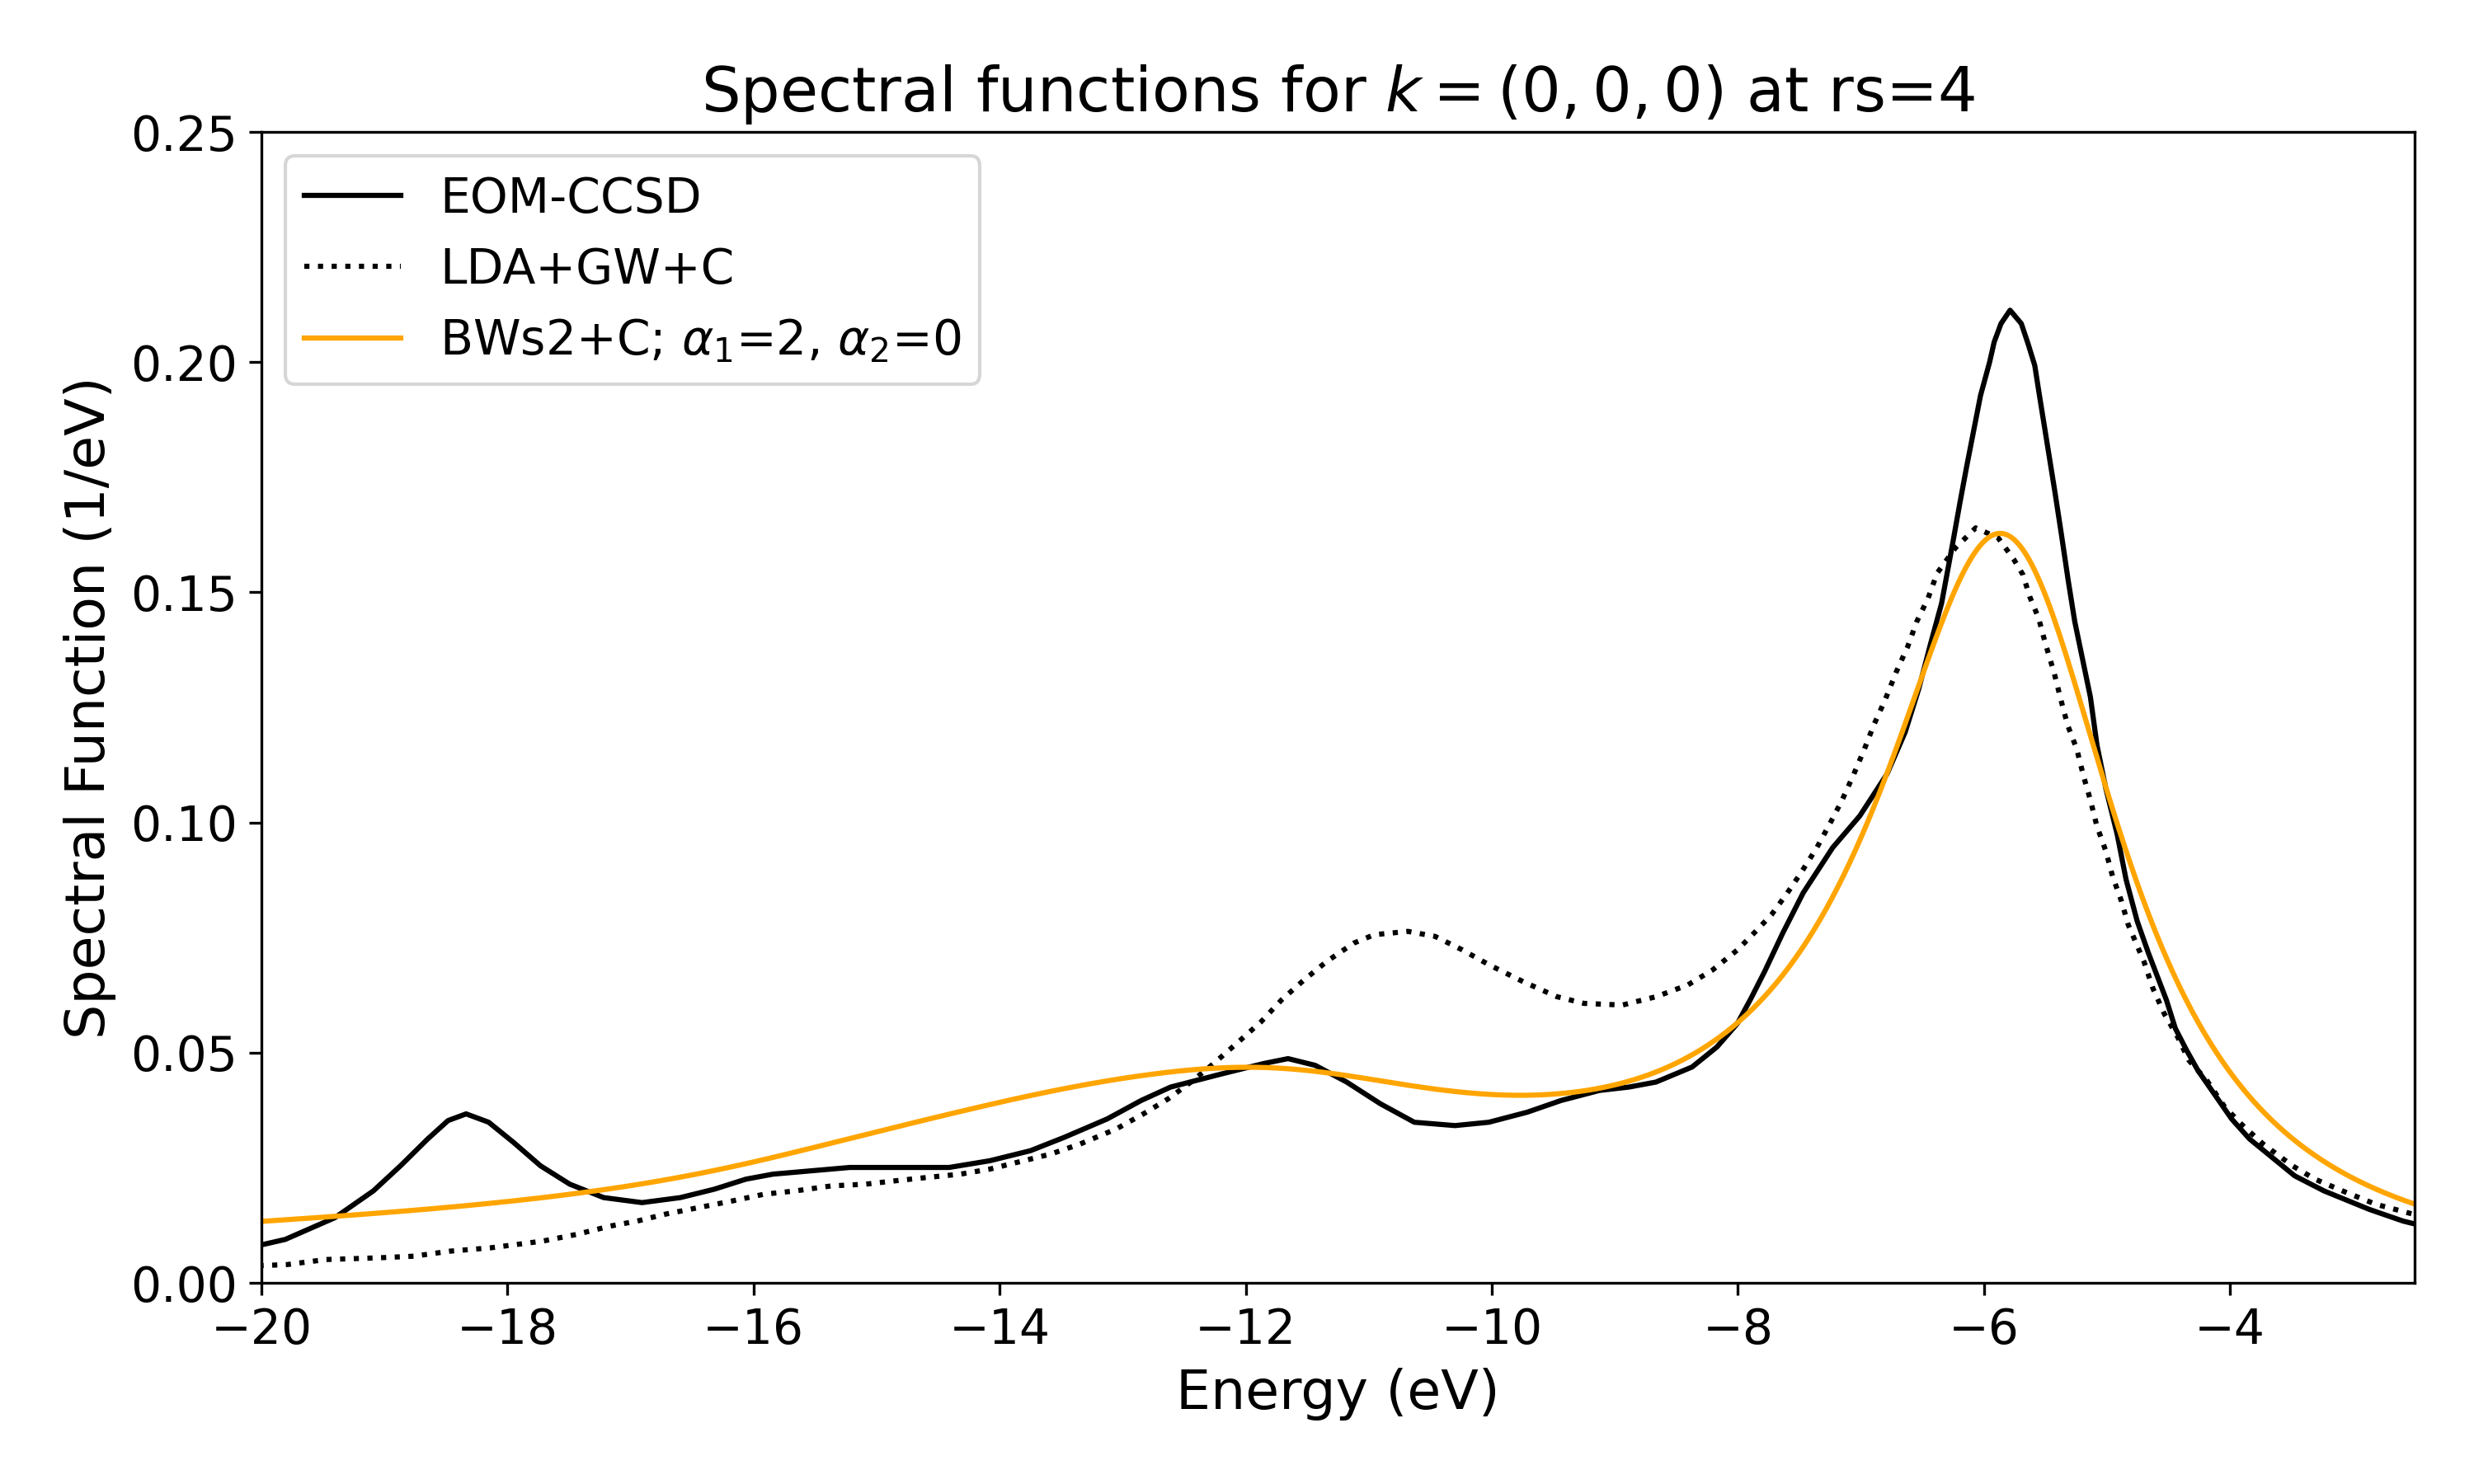
\includegraphics[width=0.75\textwidth]{../figs/bws2_pqe2_v2.png}
  \caption{Spectral functions of the UEG at the $\Gamma $ point for $r_s = 4$, which corresponds to the density of metallic sodium. Curves are shown for BWs2+C (where we set $\alpha_1 = 2$ and $\alpha_2 = 0$), GW+C ($G_0$ from DFT-LDA), and with EOM-CCSD, with the latter two reproduced from \citet{McClain2016-md}. The UEG supercell contains 114 electrons in 485 orbitals.}
  \label{fig:bws2_pqe}
\end{figure}
\section{Future directions}
\subsection{A self-consistent cumulant expansion}
Self-consistency has been incorporated into perturbative approaches for solving the Dyson equation, such as GW,
with mixed success. In these schemes, low-order diagrams are treated exactly, but higher order diagrams are neglected. Therefore, adding self consistency may lead to the double counting of terms in the expansion. Alternatively, self-consistency may be pursued within the cumulant framework. Here, although few diagrams are treated exactly, the remaining infinity are treated approximately. There have been a few studies of the self-consistent cumulant, but they have all been carried out analytically in the TDL\cite{Holm1997-by,Robinson2022-wc,Dunn1975-ew}. We propose to pursue a numerically self-consistent cumulant. This means defining a frequency grid to solve for $C^R(t)$ via equation~\ref{eq:cumulant}, which may then be used to obtain $G^R(\omega)$ via equation~\ref{eq:cumulant_G}. Then, $\Sigma^R(\omega)$ may be solved for via equation~\ref{eq:rearranged_dyson} to update $C^R(t)$, iterating until convergence.

\subsection{Memory kernel as an alternative to the self-energy}
The generalized quantum master equation (GQME) describes the time evolution of a correlation function $\mathcal{C}(t)$ as
\begin{equation}
\dot{\mathcal{C}}(t) = \mathcal{C}(t) {\Omega_1} - \int_{0}^{t} d \tau\, \mathcal{C}(t - \tau) \mathcal{K}_1(\tau) + D(t),
\label{eq:gqme}
\end{equation}
with the moment $\Omega_1$, the memory kernel $\mathcal{K}_1(t)$, and an inhomogeneous term $D(t)$\cite{Mori1965-mf}. This is to be compared with the equation of motion of the retarded Green's function, which is given by
\begin{equation}
i\partial_t G^R(t) =  \epsilon_0 G^R(t)  + \int_0^t d\tau\, \Sigma^R(t - \tau)\, G^R(\tau),
% (i\partial_t - \epsilon_0) G^R(t) - \int_0^t d\tau\, \Sigma^R(t - \tau)\, G^R(\tau) = 0 \label{eq:eom_retarded}
\end{equation}
where $\epsilon_0$ is the noninteracting quasiparticle energy. 
This implies that $\mathcal{K}_1(t)$ and $\Sigma^R(t)$ may both be used to obtain a perturbative solution to equation~\ref{eq:dyson}. However, in the former, one expands in the time variable, while in the latter, one expands in the interaction strength. The memory kernel is expected to decay quickly with time\cite{Ivander2024-fr,Du2023-kd}, while the self-energy may not decay quickly with the interaction strength\cite{Mahan2014-ad}. A symptom of the latter phenomenon is an inability of perturbative expansions in the interaction strength to adequately describe strongly correlated systems, where the interaction is large. It happens to be the case that strong correlated materials exhibit the special properties needed to accelerate materials discovery for climate change mitigation.


%%%%%%%%%%%%%%%%%%%%%%%%%%%%%%%%%%%%%%%%%%%%%%%%%%%%%%%%%%%%%%%%%%%%%
%% Start the main part of the manuscript here.
%%%%%%%%%%%%%%%%%%%%%%%%%%%%%%%%%%%%%%%%%%%%%%%%%%%%%%%%%%%%%%%%%%%%%




%%%%%%%%%%%%%%%%%%%%%%%%%%%%%%%%%%%%%%%%%%%%%%%%%%%%%%%%%%%%%%%%%%%%%
%% If you are using classical BibTeX rather than biblatex,
%% remove the \printbibliography and uncomment the \bibliograpy one
%%%%%%%%%%%%%%%%%%%%%%%%%%%%%%%%%%%%%%%%%%%%%%%%%%%%%%%%%%%%%%%%%%%%%
\newpage
\bibliography{pqe}


\end{document}
